\documentclass[11pt]{jarticle}

\usepackage{amsmath}
\usepackage{graphics}
\usepackage{hyperref}

\setlength{\oddsidemargin}{-0.7cm}
\setlength{\topmargin}{-1.5cm}
\setlength{\textwidth}{16.5cm}
\setlength{\textheight}{26cm}
\pagestyle{empty}

\begin{document}

\noindent
{\bf\large 「計算機実験II」実習課題(EX2) 2017-11-10}
\\[-0.5em]

\noindent
\begin{itemize}
\item 講義のページ: \verb+http://exa.phys.s.u-tokyo.ac.jp/ja/lectures/2017W-computer2+

\item サンプルプログラム: 「実習EX2サンプルプログラム」{\tt example-2-L2.zip}

\item モンテカルロ法とヒストグラムに関する補足資料: 「実習EX2補足資料」{\tt supplement-2-2.pdf}

\item 準備練習
  
\begin{enumerate}
\item {\tt example-2-L2/random.c}は、Mersenne-Twister 乱数発生器 (mersenne twister.h) により、(0, 1) の範囲で一様分布する実数乱数を生成するプログラムである。種(seed)を変えて何度か乱数を生成し、その時系列を比較してみよ
\item {\tt example-2-L2/histogram.c}は、$(0,1)$の一様乱数を生成し、そのヒストグラムを出力するプログラムである。コンパイル・実行し、下のようなグラフを作成してみよ
  \begin{center}
    \resizebox{.5\textwidth}{!}{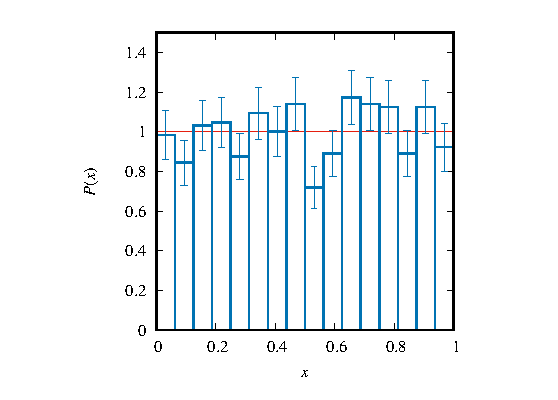
\includegraphics{histogram.eps}}
  \end{center}
\item {\tt example-2-L2/square\_lattice.c}は、二次元正方格子において、ある格子点の4つの最近接格子点を与えるプログラムである。整数除算や剰余計算({\tt \%})の使い方を確認せよ
\end{enumerate}

\item 基本課題
  \begin{enumerate}
  \item $X$と$Y$を$(0,1)$で一様分布するそれぞれ独立な(実数)確率変数とする。このとき$X^2$, $-\log X$, $XY$のそれぞれの確率密度関数と期待値を(解析的に)求めよ。また、実際に乱数を生成させてヒストグラムと期待値を計算し、解析的な結果と比較せよ
  \item 棄却法により、確率密度関数
    \begin{equation}
      P(x) = \begin{cases} 4x & 0 < x < 1/2 \\
        4(1-x) & 1/2 < x < 1 \\
        0 & \text{otherwise}
      \end{cases}
      \label{eqn:triangle}
    \end{equation}
    にしたがう一様乱数を生成せよ。ヒストグラムを作り、結果を確認せよ
  \item 確率密度関数(\ref{eqn:triangle})にしたがう$m=10$個の独立な確率変数の平均$Y=(1/m) \sum_{i=1}^m X_i$のヒストグラムを調べよ。$m$を増やしていくと分布はどのような形に近づくだろうか? 理論の予想と比較してみよ
  \item マルコフ連鎖モンテカルロ法により、二次元正方格子イジング模型のエネルギーと比熱、磁化の二乗の期待値を計算せよ。システムサイズを$L=8$, 12, 16と増やすと、これらの物理量の振る舞いがどのように変化するか調べよ
  \end{enumerate}  
\item 応用課題
  \begin{enumerate}
  \item 正規分布にしたがう乱数の生成方法について調べよ。また、平均値$\mu_i$と分散共分散行列$\Sigma_{ij}$をもつ多次元正規分布にしたがう乱数の生成方法を考えよ
  \item 一次元イジング模型の物理量は、転送行列法を用いて厳密に計算可能である。マルコフ連鎖モンテカルロ法により計算した物理量と厳密解を比較し、一致するかどうか確認してみよ。システムサイズ依存性はどのようになっているか調べよ。
  \item マルコフ連鎖モンテカルロ法により得られた、二次元正方格子イジング模型の有限系の物理量から、熱力学的極限における二次相転移の臨界温度と臨界指数を求める方法について調べよ
  \end{enumerate}

\item レポート課題No.1

  基本課題1,2,3,4についてレポートを作成し提出せよ。実習1(EX1)のレポート課題とあわせて、一つのレポート(PDF)としてITC-LMSで提出すること。提出締め切りは12月1日とする。ソースコードを全て含める必要はないが、プログラム作成時に苦労した点、工夫した点などについて適宜ソースコードを引用して説明すること
\end{itemize}

\end{document}
